%\documentclass[11pt,a4paper,titlepage,twoside]{article}
\documentclass[12pt,a4paper,twoside]{article}
\usepackage{mystyle}
\usepackage{foto_v001}
\usepackage{gplot}
\usepackage{tabelle_v001}
\usepackage{mechanik_v001}
%\usepackage{import}

\usepackage{url}

%oben und unten
\usepackage{fancyhdr}
\pagestyle{fancy}
\lhead{}
\rhead{}
\rfoot{Felix Binder}
\lfoot{Hydrostatik 2014}
\renewcommand\headrulewidth{0pt}
\renewcommand\footrulewidth{1pt}
%ende oben und unten

\date{}
%\author{Felix Binder}
\title{Hydrostatik\\{\large Die Physik von Flüssigkeiten und Gasen}}


\begin{document}
\maketitle

%\addtocounter{page}{5}
%\addtocounter{section}{9}
%\addtocounter{aufgabe}{27}


\section*{Einleitung}
Die Hydrostatik beschäftigt sich mit der Physik von Flüssigkeiten und Gasen (Fluide).
Dabei betrachten wir nur den statischen Fall, das Fluid strömt also nicht.

\section*{Die Dichte}
Die Dichte sollten Sie schon aus der Mechanik und der Chemie kennen. 
Erinnern Sie sich noch?
Sie ist wie folgt definiert:

\begin{cbox}
\begin{gather*}
	\text{Dichte} = \frac{\text{Masse}}{\text{Volumen}} \quad\text{oder}\quad \rho = \frac{m}{V}\\
	\text{Einheit}: [\rho]=\frac{\text{Kilogramm}}{\text{Kubikmeter}}=\frac{\si{kg}}{\si{m^3}}
\end{gather*}
\end{cbox}

Das Formelzeichen der Dichte $\rho$ ist ein griechischer Buchstabe. Man spricht ihn rho aus.
Wir benutzen als Einheit für die Dichte $\nicefrac{\textrm{kg}}{\textrm{m}^3}$. In der Chemie wird meistens die
Einheit $\nicefrac{\textrm{g}}{\textrm{cm}^3}$ verwendet.

\begin{aufgabe}
	Rechnen Sie die Dichte von \SI{2.7}{g/cm^3} in die in der Physik gebräuchliche Einheit $\nicefrac{\textrm{kg}}{\textrm{m}^3}$ um.

	\kloesung{\SI{2700}{kg/m^3}}

	\begin{loesung}
		\begin{eqnarray*}
			\SI{2.7}{g/cm^3} = \num{2.7}\frac{\SI{1E-3}{kg}}{(\SI{1E-2}{m})\cdot(\SI{1E-2}{m})\cdot(\SI{1E-2}{m})}=\num{2.7}\frac{\SI{1E-3}{kg}}{\SI{1E-6}{m^3}}=\SI{2.7E3}{kg/m^3}=\SI{2700}{kg/m^3}
		\end{eqnarray*}
	\end{loesung}

\end{aufgabe}

\begin{aufgabe}
Bestimmen Sie die Dichte der Schüler im Klassenraum.
Welche maximale Dichte ist möglich? Wie kann man diese bestimmen?
\end{aufgabe}


Wir bestimmen nun die Dichte von Wasser und anschliessend die Dichte eines Steins. 
Bitte machen sie Vorschläge wie man das machen könnte.\par


\begin{aufgabe}
	Bestimmen Sie das Volumen von \SI{1}{kg} Gold. Welche Kantenlänge hat ein Würfel mit diesem Volumen?
	\begin{loesung}
		Zuerst bestimmen wir das Volumen:
		\begin{eqnarray*}
			\rho=\frac{m}{V}\to V=\frac{m}{\rho}=\frac{\SI{1}{kg}}{\SI{19290}{kg/m^3}}=\SI{5.1840e-05}{m^3}
		\end{eqnarray*}
		Für einen Würfel gilt: $V=a^3\to a=\sqrt[3]{V}=\SI{0.037287}{m}\approx\SI{3.7}{cm}$.
	\end{loesung}
	\kloesung{$a\approx\SI{3.7}{cm}$}
\end{aufgabe}
\Karo{2}

\begin{aufgabe}
	Vervollständigen Sie die Tabelle.

	\begin{tikzpicture}
	
	\matrix (A) [Tabelle,text width=10em]
{
      &                    &                &\\
      & \SI{7.86}{g/cm^3}  & \SI{200}{cm^3} & \\
      & \SI{13.55}{g/cm^3} &                & \SI{0.7}{kg} \\
Gold  &                    & \SI{200}{cm^3} & \\
Wasser&                    &                & \SI{0.7}{kg} \\
};
\end{tikzpicture}

\begin{loesung}


	\begin{tikzpicture}
	
	\matrix (A) [Tabelle,text width=10em]
{
Material      & Dichte             &   Volumen      & Masse\\
Eisen         & \SI{7.86}{g/cm^3}  & \SI{200}{cm^3} & \SI{1.572}{kg}\\
Quecksilber   & \SI{13.55}{g/cm^3} &\SI{51.66}{cm^3}& \SI{0.7}{kg} \\
Gold          & \SI{19.29}{g/cm^3} & \SI{200}{cm^3} & \SI{3.858}{kg}\\
Wasser        & \SI{1}{g/cm^3}     & \SI{700}{cm^3} & \SI{0.7}{kg} \\
};
\end{tikzpicture}
	
\end{loesung}

\end{aufgabe}


\subsection*{Die Dichte der Luft}
\begin{aufgabe}
	Wie kann man die Dichte von Luft messen?
	Überlegen Sie sich eine Methode und beschreiben Sie die nötigen Schritte.
\end{aufgabe}

\begin{aufgabe}
	Bestimmen Sie grob die Masse der Luft im Physikraum. 
\end{aufgabe}


\begin{aufgabe}
	Wie viele Luftballons mit \SI{5}{Litern} Füllvolumen können mit \SI{100}{kg} Helium gefüllt werden
	(bei normalem Luftdruck und \SI{0}{\celsius} Temperatur)?

	\begin{loesung}
		Das Volumen von \SI{100}{kg} Helium bei Normalbedingungen berechnet sich so:
		\begin{eqnarray*}
			\rho=\frac{m}{V}\to V=\frac{m}{\rho}=\frac{\SI{100}{kg}}{\SI{0.1768}{kg/m^3}}=\SI{565.61}{m^3}
		\end{eqnarray*}

		Ein Luftballon hat ein Volumen von $\SI{5}{l} = \SI{5}{dm^3} = \SI{5E-3}{m^3}$.
		Es lassen sich also $\nicefrac{V}{\RI{V}{Ballon}}$ Luftballons füllen.
		Das macht \SI{113122} Luftballons.

	\end{loesung}

\end{aufgabe}
\Karo{2}

\newpage
\subsection*{Dichtetabelle $\rho$ [kg/m$^3$]}
\usetikzlibrary{positioning}
\begin{center}
\begin{tikzpicture}
%	\node [rectangle, text width=20em](oben){Dichtetabelle\\Die Werte für Gase gelten bei \SI{0}{\celsius}};
	
	%\matrix (links) [below = of oben,Tabelle,text width=10em]
	\matrix (links) [left,Tabelle,text width=10em]
{
Aluminium & 2700 \\
Blei      & 11340\\
Eisen     &  7860\\
Gold      & 19290\\
Kupfer    & 8920 \\
Nickel    & 8900 \\
Platin    & 21450\\
Silber    & 10500\\
Zink      & 7140 \\
          &      \\
Beton     & ca. 2000 \\
Glas      & ca. 2600\\
Plexiglas & 1190\\
Messing   & ca. 8400\\
Stahl     & ca. 7900\\
Holz      & 500 - 700\\
Kork      & ca. 300\\
Eis (\SI{0}{\celsius} & 917 \\
};
%\matrix (rechts) [below= of oben, Tabelle,text width=10em]
\matrix (rechts) [right, Tabelle,text width=10em]
{
Äther     & 714 \\
Alkohol   & 789\\
Olivenöl  & 914\\
Petroleum & 850\\
Quecksilber  & 13546 \\
&  \\
Wasser \SI{0}{\celsius}    & \num{999.84}\\
Wasser \SI{4}{\celsius}    & \num{999.97}\\
Wasser \SI{100}{\celsius}    & \num{958.35}\\
    & \\
	Chlorgas      & \num{3.214} \\
	Helium        & \num{0.1768}\\
	Kohlendioxid  & \num{1.9769} \\
	Luft  & \num{1.2929} \\
	Methan  & \num{0.7168} \\
	Sauerstoff  & \num{1.429} \\
	Stickstoff  & \num{1.2505} \\
	Wasserstoff  & \num{0.0899} \\
	};

\end{tikzpicture}

Die Werte der Gase gelten bei \SI{0}{\celsius}.
\end{center}
	

\newpage



\section*{Der hydrostatische Druck}
Der Druck in Flüssigkeiten und Gasen wird hydrostatischer Druck genannt.
Dieser Druck wirkt in alle Raumrichtungen gleich. Um den Grund dafür zu verstehen,
muss man sich das Fluid (Flüssigkeit oder Gas) aus Atomen oder Molekülen vorstellen.
Diese Teilchen schwingen im Fluid und bewegen sich ungeordnet in alle Richtungen.
Dabei üben sie eine Kraft aus, die in Bewegungsrichtung zeigt. Im Mittel wird also
in alle Raumrichtungen die gleiche Kraft ausgeübt. Dadurch ist auch der Druck $P$ in alle
Raumrichtungen gleich.

Der Druck in einem Fluid wird mit steigender Tiefe höher. Als Beispiel können wir den Wasserdruck
beim Tauchen betrachten. Während wir an der Wasseroberfläche den Druck nicht spüren, steigt dieser
mit zunehmender Tauchtiefe. Gleichzeitig steigt das Gewicht (die Gewichtskraft) des Wassers über
unserem Körper.

Im folgenden wollen wir den Wasserdruck ($P_{\textrm w}$) in Abhängigkeit zur Wassertiefe herleiten:

\begin{equation*}
	P_{\textrm w} = \frac{F_{\textrm G}}{A}=\frac{m\cdot g}{A}=\frac{\overbrace{\rho_{\textrm w} \cdot V}^{m} \cdot g}{A}=\frac{\rho_{\textrm w} \cdot \overbrace{A \cdot h}^{V} \cdot g}{A}=\rho_{\textrm w}\cdot g\cdot h.
\end{equation*}

Dabei ist $F_{\textrm G}$ die Gewichskraft, $A$ die Fläche, $\rho_{\textrm w}$ die Dichte von Wasser, $V$ das Volumen und $h$
die Wassertiefe.

Zusammenfassend kann man schreiben:
\begin{cbox}
	\begin{eqnarray*}
	P_{\textrm w} = \rho_{\textrm w}\cdot g\cdot h.
	\end{eqnarray*}
\end{cbox}

Die Formel sagt aus, dass der Wasserdruck nur von der Wassertiefe abhängt (Wasserdichte und Fallbeschleunigung sind konstant)
und nicht von der Form des Behälters.
Dieser einfache Ausdruck für den Wasserdruck beruht auf der Annahme, dass die Wasserdichte unabhängig vom
Wasserdruck konstant ist. Dies gilt näherungsweise für alle Flüssigkeiten. In Gasen ist diese einfache
Annahme nicht gültig.

Übt man auf die Wasseroberfläche einen zusätzlichen Druck $P_0$ aus kann man diesen zum Wasserdruck $P_{\textrm w}$ addieren
und erhält dann den Gesamtdruck $P$.

\begin{cbox}
	\begin{equation*}
		P = P_0 + P_{\textrm w} = P_0 + \rho \cdot g \cdot \Delta h
	\end{equation*}
\end{cbox}

%nicht so eine gute aufgabe für den Anfang
%\begin{aufgabe}
%	Wie tief muss man Tauchen, damit sich der Druck im Vergleich zur Wasseroberfläche
%verdoppelt?
%\begin{loesung}
%	Druck an der Wasseroberfläche ist etwa \SI{1000}{hPa}.
%	\begin{equation*}
%		P = \rho_{\textrm w} \cdot g \cdot h \to h = \frac{P}{\rho_{\textrm w}\cdot g}=\frac{\SI{1E5}{Pa}}{\SI{1000}{kg/m^3} \cdot \SI{10}{N/kg}} = \SI{10}{m}
%	\end{equation*}
%\end{loesung}
%\kloesung{\SI{10}{m}}
%\end{aufgabe}

\begin{aufgabe}
	Wie hoch ist der Wasserdruck bei a) \SI{3}{m} b) \SI{2000}{m} Wassertiefe?
	\begin{loesung}
	\begin{itemize}
		\item[a)]
			\begin{eqnarray*}
				P=\rho_{\textrm w}\cdot g\cdot h=\SI{1000}{kg/m^3}\cdot\SI{10}{N/kg}\cdot\SI{3}{m}=\SI{30000}{Pa}
			\end{eqnarray*}
		\item[b)]
			\begin{eqnarray*}
				P=\rho_{\textrm w}\cdot g\cdot h=\SI{1000}{kg/m^3}\cdot\SI{10}{N/kg}\cdot\SI{2000}{m}=\SI{20000000}{Pa}
			\end{eqnarray*}
	\end{itemize}
\end{loesung}
\kloesung{a) \SI{30000}{Pa} und b) \SI{20000000}{Pa}}

\end{aufgabe}

\begin{aufgabe}
	Die Staumauer Grand Dixence im Wallis ist eine der höchsten Staumauern der Welt.
	Die maximale Höhe beträgt \SI{285}{Meter}, die maximale ``Dicke'' am Fuss \SI{198}{Meter}.
	In der achtjährigen Bauzeit wurden sechs Millionen Kubikmeter Beton verarbeitet.
	\begin{enumerate} [a)]
		\item Warum spielte die Form und Länge des Stausees keine Rolle für die Dimensionalisierung der Mauer?
		\item Musste der Luftdruck bei der Bestimmung der Mauerbeanspruchung berücksichtigt werden?
	\end{enumerate}

	\begin{loesung}
		\begin{enumerate} [a)]
			\item Für die Dimensionierung der Mauer muss der Druck auf die Mauer berücksichtigt werden.
				Der Wasserdruck ist unabhängig von der Form des Wassergefässes, auch bei Seen.
				Einzig der Wasserstand also die Höhe des Wassers hat einen Einfluss auf den Druck.
			\item Nein. Der Luftdruck musste nicht berücksichtigt werden. Der Luftdruck drückt zwar auf die
				Wasseroberfläche des Sees, der Druck im See ist damit höher als ohne den Luftdruck, aber
				der Luftdruck drückt auch gegen die Staumauer und stützt diese dadurch.
				Effektiv gleichen sich beide Effekte aus.
		\end{enumerate}
	\end{loesung}


\end{aufgabe}

\begin{aufgabe}
	Welche Kraft wirkt auf einen Qudratzentimer der Körperoberfläche einer Taucherin in \SI{50}{m} Tiefe?
	Der Luftdruck beträgt \SI{960}{hPa}.
	\begin{loesung}
		Der Druck in \SI{50}{m} Wassertiefe ist die Summe aus Luftdruck an der Oberfläche und Wasserdruck in \SI{50}{m} Tiefe.
		\begin{eqnarray*}
			P = P_0 + P_{\textrm w} = P_0 + \rho \cdot g \cdot \Delta h=\SI{960}{hPa}+\SI{1000}{kg/m^3}\cdot\SI{10}{m/s^2}\cdot\SI{50}{m}=\SI{5960}{hPa}
		\end{eqnarray*}
		Druck ist der Quotient aus Kraft $F$ und Fläche $A$
		\begin{eqnarray*}
			P=\frac{F}{A}\to F=P\cdot A=\SI{5960}{hPa}\cdot\SI{1E-4}{m^2}=\SI{59.6}{N}
		\end{eqnarray*}
	\end{loesung}
	\kloesung{\SI{59.6}{N}}
\end{aufgabe}

\newpage
\section*{Druckmessung}
Für die Druckmessung verwendet man Manometer (Druckmesser). Heutige Manometer funktionieren meistens
elektronisch. Hier wollen wir zwei Flüssigkeitsmanometer kennenlernen.
Das erste ist das offene U-Rohr-Manometer. Es besteht aus einem U-förmigen Rohr, das etwa halb mit einer Flüssigkeit
gefüllt ist. Herrscht auf beiden Seiten des U-Rohrs der gleiche Druck, so ist die Oberfläche auf der linken Seite
auf gleicher Höhe wie die Oberfläche auf der rechten Seite des U-Rohrs.
Wird auf einer Seite ein Überdruck ($P_{\textrm e}$) angelegt, so verschieben sich die Oberflächen gegeneinander.
Mit diesem Manometer kann man nur Druckdifferenzen messen.

\begin{minipage}{0.5\textwidth}
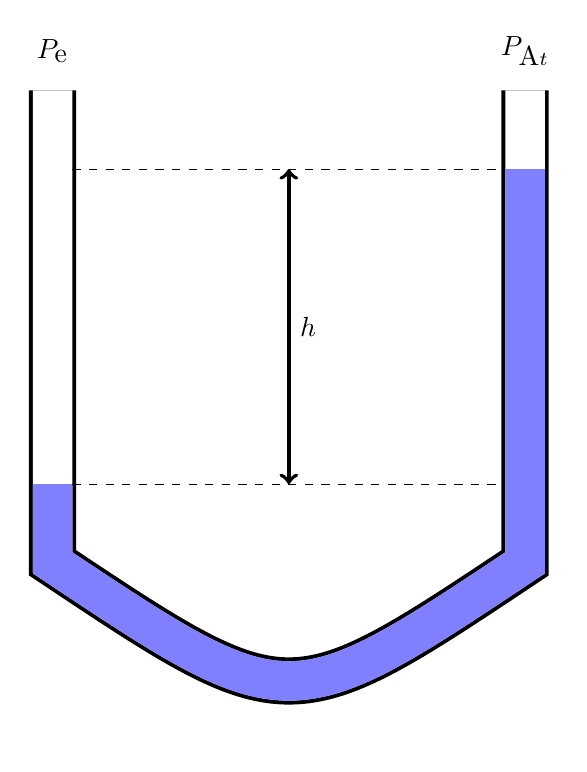
\begin{tikzpicture}[info text/.style={rounded corners, fill=red!20, inner sep=1ex}]
%\begin{tikzpicture}
\usetikzlibrary{calc,intersections,through,backgrounds}
\usetikzlibrary{decorations.pathmorphing}
%\draw[step=0.5cm,lightgray] (-0.5,-3.0) grid (6.5,5.0);

\draw [double distance=0.5cm, line width=0.05cm] (0,5)--(0,-1)..controls (3,-3) .. (6,-1)--(6,5);
\draw [line width=0.5cm,color=blue!50] (0,0)--(0,-1)..controls (3,-3) .. (6,-1)--(6,4);

\draw [dashed] (0.25,0)--(5.75,0);
\draw [dashed] (0.25,4)--(5.75,4);

%beschriftung der Höhe
\draw [<->, line width=0.05cm] (3,0)--(3,4);
\node at (3,2) [line width=0.05cm, right] {$h$};

%beschriftung Druck
\node at (6,5.5) {$P_{\textrm At}$};
\node at (0,5.5) {$P_{\textrm e}$};

\end{tikzpicture}
\end{minipage}
\begin{minipage}{0.5\textwidth}
Mit dem Höhenunterschied zwischen den beiden Oberflächen kann der Überdruck bestimmt werden. Es gilt


\begin{cbox}
	\begin{eqnarray*}
		P_{\textrm e}= \rho\cdot g\cdot h.
	\end{eqnarray*}
\end{cbox}

Dabei ist $\rho$ die Dichte der Flüssigkeit im inneren des U-Rohrs, $g$ die Fallbeschleunigung und $h$ der Höhenunterschied
zwischen beiden Oberflächen.
\end{minipage}


Heute sind diese Manometer nicht mehr sehr verbreitet.
Historisch wurde das offene Quecksilber Manometer zur Messung des Blutdrucks verwendet.
Die Einheit des Blutdrucks ist bis heute mmHg, also der Höhenunterschied von Quecksilber (Hg)
in einem offenen U-Rohr-Manometer.

\begin{aufgabe}
	\begin{itemize}
		\item[a)] Wie hoch ist der Druck von \SI{120}{mmHg} in der für den Druck üblichen Einheit Pascal?
		\item[b)] Welchem Höhenunterschied entspricht dass, wenn stattdessen Wasser im Manometer verwendet wird?
	\end{itemize}

	\begin{loesung}
	\begin{itemize}
		\item[a)]
		\begin{eqnarray*}
			P=\rho_{\textrm Hg}\cdot g\cdot h = \SI{13546}{kg/m^3}\cdot \SI{10}{N/kg}\cdot\SI{0.12}{m}=\SI{1.6255e+4}{Pa}
		\end{eqnarray*}
	\item[b)]
		\begin{eqnarray*}
			P=\rho\cdot g\cdot h \to h= \frac{P}{\rho\cdot g}=\frac{\SI{1.6255E4}{Pa}}{\SI{1000}{kg/m^3}\cdot \SI{10}{N/kg}}=\SI{1.63}{m}
		\end{eqnarray*}

\end{itemize}
	\end{loesung}
\end{aufgabe}

Eine Variation des offenen Manometers ist das geschlossene Manometer. Mit diesem werden keine Druckdifferenzen gemessen,
wie beim offenen Manometer sondern absolute Drücke.

\begin{minipage}{0.5\textwidth}
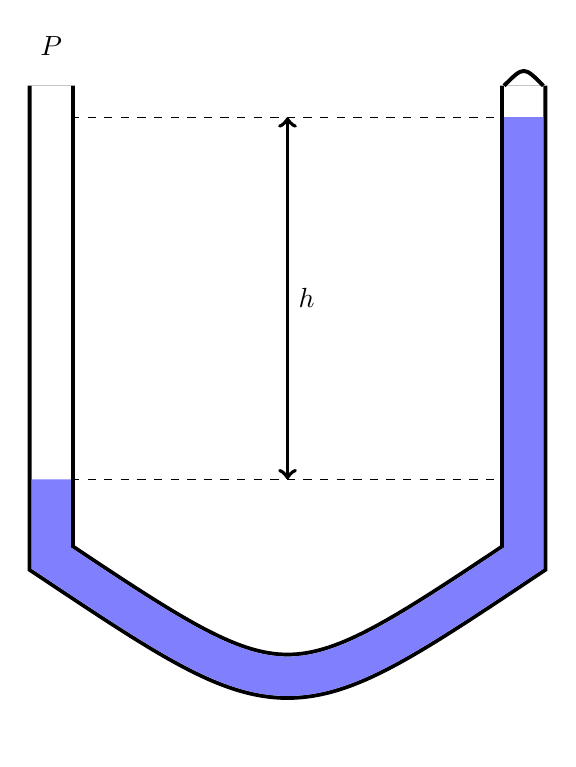
\begin{tikzpicture}[info text/.style={rounded corners, fill=red!20, inner sep=1ex}]
%\begin{tikzpicture}
\usetikzlibrary{calc,intersections,through,backgrounds}
\usetikzlibrary{decorations.pathmorphing}
%\draw[step=0.5cm,lightgray] (-0.5,-3.0) grid (6.5,5.0);

\draw [double distance=0.5cm,line width=0.05cm] (0,5)--(0,-1)..controls (3,-3) .. (6,-1)--(6,5);
\draw [line width=0.05cm] (5.75,5)..controls (6,5.25)..(6.25,5);

\draw [line width=0.5cm,color=blue!50] (0,0)--(0,-1)..controls (3,-3) .. (6,-1)--(6,4.6);

\draw [dashed] (0.25,0)--(5.75,0);
\draw [dashed] (0.25,4.6)--(5.75,4.6);

%beschriftung der Höhe
\draw [<->, line width=0.05cm] (3,0)--(3,4.6);
\node at (3,2.3) [line width=0.05cm, right] {$h$};

%beschriftung Druck
%\node at (6,5.5) {$P_{\textrm At}$};
\node at (0,5.5) {$P$};

\end{tikzpicture}
\end{minipage}
\begin{minipage}{0.5\textwidth}

	Mit dem Höhenunterschied zwischen den beiden Oberflächen kann der Druck bestimmt werden. Es gilt


\begin{cbox}
	\begin{eqnarray*}
		P= \rho\cdot g\cdot h.
	\end{eqnarray*}
\end{cbox}

Dabei ist $\rho$ die Dichte der Flüssigkeit im inneren des U-Rohrs, $g$ die Fallbeschleunigung und $h$ der Höhenunterschied
zwischen beiden Oberflächen.
In der geschlossenen Röhre bildet sich oben ein Vakuum. Im Vakuum ist der Druck Null. Deshalb kann
in diesem Manometer der Druck gemessen werden.
\end{minipage}
Historisch wird dieser Manometertyp zur Messung des Luftdrucks verwendet.
Der Normaldruck von \SI{1013}{hPa} entspricht einer Quecksilbersäule von \SI{76}{cm}.

\begin{aufgabe}
	In einem Experiment sehen Sie ein geschlossenes Quecksilbermanometer unter einer Glasglocke.
	Mit der Vakuumpumpe wird die Luft aus der Glasglocke gepumpt.
	Lesen Sie den Höhenunterschied zwischen den zwei Flüssigkeitsoberflächen ab und bestimmen Sie den Druck unter der Glasglocke.
\end{aufgabe}

\newpage
\section*{Der Luftdruck}

\begin{aufgabe}
	Lesen Sie den Ausschnitt zum Barometer aus der Wikipedia und beantworten Sie folgende Fragen:
	\begin{enumerate} [a)]
		\item Was ist ein Barometer?
		\item Welche Funktion hat das Barometer?
		\item Skizzieren Sie die geschichtliche Entwicklung des Barometers.
		\item Was wurde mit dem Barometer erforscht?
		\item Beschreiben Sie das Funktionsprinzip des Barometers.
		\item Was hat Ihnen besonders gut an dem Artikel gefallen?
	\end{enumerate}
\end{aufgabe}


\begin{aufgabe}
	In der Physiksammlung gibt es ein Quecksilberbarometer. Gehen Sie in kleinen Gruppen (maximal drei Personen)
	und schauen Sie es sich an. Lesen Sie die Höhe der Quecksilbersäule ab.
	Berechnen Sie am Arbeitsplatz den heutigen Luftdruck.
\end{aufgabe}

\begin{aufgabe}
	\label{konstanteDichte}
	Nehmen Sie an, die Dichte der Luft in der Atmosphäre ist nicht abhängig von der Höhe, 
	sondern konstant die Dichte bei Normalbedingungen.
	Bis wohin reicht die Atmosphäre in diesem Fall?
	
	\kloesung{\SI{7943}{m}}

	\begin{loesung}
	In dieser Aufgabe wird angenommen, dass die Luft nicht komprimiert werden kann.
	Die Luft soll sich also wie eine Flüssigkeit verhalten.
	\begin{eqnarray*}
		P=\rho\cdot g\cdot h\to h=\frac{P}{\rho\cdot g}=\frac{\SI{101300}{Pa}}{\SI{1.3}{kg/m^3}\cdot\SI{9.81}{m/s^2}}=\SI{7943.22}{m}
	\end{eqnarray*}
	\end{loesung}

\end{aufgabe}

\begin{aufgabe}
	In Aufgabe \ref{konstanteDichte} haben Sie angenommen, die Dichte der Luft sei über die gesamte Atmosphäre konstant.
	Verbessern Sie dieses Modell, indem Sie die Atmosphäre in \SI{1}{km} Dicke schichten konstanter Dichte zerlegen.
	\begin{enumerate}[a)]
		\item Welcher Luftdruck ergibt sich für \SI{5}{km} bzw.~\SI{10}{km} über dem Meer, wenn Sie von Normalbedingungen
			und konstanter Temperatur auf Meereshöhe ausgehen? 
		\item Vergleichen Sie die Werte aus a) mit der barometrischen Höhenformel:
			\begin{eqnarray*}
				P&=P_0\cdot e^{-\frac{\rho_0 g}{P_0}\cdot h}
			\end{eqnarray*}
	\end{enumerate}
	\kloesung{a) \SI{517}{hPa} und \SI{264}{hPa}, b) \SI{540}{hPa} und \SI{288}{hPa}}
	
\end{aufgabe}


%\begin{aufgabe}
%	An einem geschlossenes Quecksilbermanometer misst man einen Höhenunterschied von \SI{74.2}{cm}.
%	Welchem Druck entspricht das in Pascal?
%	\begin{loesung}
%	\begin{eqnarray*}
%		P=\rho_{\textrm Hg}\cdot g\cdot h = \SI{13546}{kg/m^3}\cdot \SI{9.81}{N/kg}\cdot\SI{0.742}{m}=\SI{98602}{Pa}=\SI{986}{hPa}
%	\end{eqnarray*}
%	\end{loesung}
%\end{aufgabe}


\newpage
\subsection*{Die Magdeburger Halbkugeln}
Im Jahre 1654 hat Otto von Guericke in Magdeburg (Deutschland) zum ersten Mal sein später berühmt gewordenes Experiment vorgeführt.
Es ist ein Experiment um die Wirkung des Luftdrucks zu verdeutlichen.
Zwei Halbkugeln werden so aneinander gelegt, dass sie eine Kugel formen.
Dann wird die Luft aus dem inneren der Kugel gepumpt. Der äussere Luftdruck drückt weiterhin auf die zwei Halbkugeln.
Dies verhindert, dass man die Halbkugeln voneinander trennen kann. Der Durchmesser der zwei Halbkugeln betrug damal \SI{42}{cm}
und 16 Pferde waren nicht in der Lage sie zu trennen.

\begin{center}
\Bildeinbinden{./83_Guericke_D.jpg}{0.9}
\end{center}

\begin{aufgabe}
	Machen Sie sich eine Skizze des Experiments und zeichnen Sie die wirkenden Kräfte ein.
Berechnen Sie, wie gross die Kräfte sein müssten um die zwei Halbkugeln zu trennen.

\begin{loesung}
	Die Fläche eines Kreises mit einem Durchmesser von \SI{42}{cm} ist:
	\begin{eqnarray*}
		A=r^2\cdot \pi=(\SI{0.21}{m})^2\cdot\pi=\SI{0.13854}{m^2}.
	\end{eqnarray*}
	\begin{eqnarray*}
		P=\frac{F}{A} \to F=P\cdot A=\SI{1E5}{Pa}\cdot\SI{0.139}{m^2}=\SI{13900}{N}
	\end{eqnarray*}
\end{loesung}
\end{aufgabe}


\newpage
\subsection*{Hydraulische Systeme}
In täglichen Leben werden häufig hydraulische Systeme benutzt, um Kräfte zu verstärken.
Ein Beispiel ist der hydraulische Wagenheber. Die Abbildung zeigt zwei Kolben, die
mit einer Flüssigkeit verbunden sind.
Erhöht man den Druck in einer Flüssigkeit indem man mit einem Kolben eine Kraft auf die
Oberfläche ausübt, so erhöht sich der Druck gleichmässig in der gesamten Flüssigkeit.

\begin{minipage}{0.5\textwidth}
\begin{tikzpicture}[info text/.style={rounded corners, fill=red!20, inner sep=1ex}]
%\begin{tikzpicture}
%\usetikzlibrary{calc,intersections,through,backgrounds}
%\usetikzlibrary{decorations.pathmorphing}
%\draw[step=0.5cm,lightgray] (-0.5,-3.0) grid (6.5,5.0);

\path[draw,fill=blue!50,line width=0.1cm] (0,0)--(0,-6)--(6,-6)--(6,0)--(3,0)--(3,-5)--(1.5,-5)--(1.5,0)--cycle;
\draw [line width=0.1 cm] (0,0)--(0,1);
\draw [line width=0.1 cm] (1.5,0)--(1.5,1);
\draw [line width=0.1 cm] (6,0)--(6,1);
\draw [line width=0.1 cm] (3,0)--(3,1);

%zylinder klein
\path[draw, fill=red!50] (0.05,-0.5)--(0.05,2)--(1,2)--(1.45,2)--(1.45,-0.5)--cycle;

%zylinder gross
\path[draw, fill=red!50] (3.05,-0.25)--(3.05,2.25)--(5.95,2.25)--(5.95,-0.25)--cycle;

\draw[<-,Kraft] (0.75,2)--(0.75,3) node [above] {$\vec{F_1}$};
\draw[->,Kraft] (4.5,2.25)--(4.5,5) node [above] {$\vec{F_2}$};

\draw[<-,line width=0.05cm] (0.75,-0.5)--++(240:2) node [below] {$A_1$};
\draw[<-,line width=0.05cm] (4.5,-0.25)--++(-60:2) node [below] {$A_2$};



\end{tikzpicture}
\end{minipage}
\begin{minipage}{0.5\textwidth}
Wird auf den linken Kolben eine Kraft $F_1$ ausgeübt, dann steigt der Druck in der Flüssigkeit. Der Druckanstieg
ist
\begin{eqnarray*}
	P = \frac{F_1}{A_1}.
\end{eqnarray*}

Der Druck in der Flüssigkeit drückt nun auf den zweiten Kolben mit der Fläche $A_2$. Dies bewirkt eine Kraft $F_2$
\begin{align*}
	F_2 &= P\cdot A_2\\
	&=\frac{F_1}{A_1}\cdot A_2\\
	&=\frac{A_2}{A_1}\cdot F_1
\end{align*}

\end{minipage}
\begin{aufgabe}
	Die zwei Kolben eines Wagenhebers haben einen Durchmesser von \SI{2}{cm} und \SI{8}{cm}.
	Wie gross ist die Kraftverstärkung?

	\begin{loesung}
		\begin{gather*}
			A_1=r^2\cdot\pi=(\SI{0.01}{cm})^2\cdot \pi=\SI{0.0001}{m^2}\cdot \pi\\
			A_2=r^2\cdot\pi=(\SI{0.04}{cm})^2\cdot \pi=\SI{0.0016}{m^2}\cdot \pi\\
		\end{gather*}
		Die Kraftverstärkung ist $A_2/A_1=16$.
	\end{loesung}
\end{aufgabe}



\newpage

\section*{Auftrieb und archimedisches Prinzip}
Wenn ein schwerer Körper an einer Feder aufgehängt und in Wasser eingetaucht wird, dann
zeigt die Skala an der Federwaage eine geringere Gewichtskraft an, als wenn der Körper
in Luft gewogen würde. Ursache dafür ist eine nach oben gerichtete Kraft, die von dem Wasser
auf den Körper ausgeübt wird und einen Teil der Gewichtskraft kompensiert. Dieses Phänomen
heisst Auftrieb. Der Auftrieb ist noch besser sichtbar, wenn man beispielsweise einen
Korken in Wasser eintaucht. Wenn er vollständig in Wasser eingetaucht ist, dann erfährt 
der Korken aufgrund des Wasserdrucks eine aufwärts gerichtete Kraft, die grösser ist
als seine Gewichtskraft. Diese Kraft, die das Fluid auf einen ganz oder teilweise eingetauchten
Körper ausübt, wird als Auftriebskraft $F_{\textrm A}$ bezeichnet. Sie hängt nicht von der Form
oder Dichte des Körpers ab, sondern nur von der Dichte des Fluids. Ihr Betrag ist gleich Gewichtskraft der
durch den Körper verdrängten Fluidmenge.

\begin{cbox}
Ein Körper, der ganz oder teilweise in ein Fluid eintaucht, erfährt eine Auftriebskraft,
deren Betrag gleich der Gewichtskraft der durch den Körper verdrängten Fluidmenge ist.

\begin{gather*}
	\text{Auftriebskraft} = \text {Fluiddichte} \cdot \text{Fallbeschleunigung}\cdot\text{Volumen}\\
	\RI{F}{A} = \RI{\rho}{w} \cdot g \cdot V
\end{gather*}
\end{cbox}

\begin{aufgabe}
	Was versteht man unter Auftrieb? Wovon hängt der Auftrieb ab?
	\begin{loesung}
		Auftrieb tritt in Flüssigkeiten und Gasen auf und beschreibt eine nach oben gerichtete Kraft.
		Die Auftriebskraft hängt von der Dichte des Fluids und vom Volumen des eingetauchten Körpers ab.
	\end{loesung}
\end{aufgabe}

\begin{aufgabe}
	Wie gross ist der Auftrieb den ein Körper mit einem Volumen von \SI{0.25}{m^3} in Wasser erfährt?
	\kloesung{\SI{2452.5}{N}}
	\begin{loesung}
		\begin{eqnarray*}
			\RI{F}{A} = \RI{\rho}{w} \cdot g \cdot V=\SI{1000}{kg/m^3}\cdot\SI{9.81}{m/s^2}\cdot\SI{0.25}{m^3}=\SI{2452.5}{N}
		\end{eqnarray*}
	\end{loesung}
\end{aufgabe}

\begin{aufgabe}
	Ein Taucher ist im Urlaub am Toten Meer ($\rho=\SI{1240}{kg/m^3}$) und möchte tauchen gehen. 
	Daheim taucht er gewöhnlich in einem Süsswassersee.
	\begin{enumerate} [a)]
		\item Was sollte der Taucher beachten?
		\item Wie viel grösser ist der Auftrieb im Toten Meer im Vergleich zum heimischen See?
	\end{enumerate}
	\kloesung{b) \num{1.24}}
	\begin{loesung}
		\begin{enumerate} [a)]
		\item Die Dichte des Wassers im Toten Meer ist höher als im Süsswassersee.
			Dadurch ist die Auftriebskraft grösser.
		\item
			\begin{eqnarray*}
				\frac{\RI{F}{A}(\textrm{Totes Meer})}{\RI{F}{A}(\textrm{Süsswassersee})}=\frac{\RI{\rho}{w}(\textrm{Totes Meer})\cdot g\cdot V}{\RI{\rho}{w}(\textrm{Süsswasser})\cdot g\cdot V}=\frac{\RI{\rho}{w}(\textrm{Totes Meer})}{\RI{\rho}{w}(\textrm{Süsswasser})}=\frac{\SI{1240}{kg/m^3}}{\SI{1000}{kg/m^3}}=\num{1.24}
			\end{eqnarray*}
		\end{enumerate}
	\end{loesung}

\end{aufgabe}


\newpage

\subsection*{Die Entdeckung des archimedischen Prinzips}
Quelle: \url{http://de.wikipedia.org/wiki/Archimedisches_Prinzip}

Archimedes war von König Hieron II. von Syrakus beauftragt worden, herauszufinden, 
ob dessen Krone wie bestellt aus reinem Gold wäre oder ob das Material durch billigeres Metall gestreckt worden sei. 
Diese Aufgabe stellte Archimedes zunächst vor Probleme, da die Krone natürlich nicht zerstört werden durfte.

Der Überlieferung nach hatte Archimedes schließlich den rettenden Einfall, 
als er zum Baden in eine bis zum Rand gefüllte Wanne stieg und dabei das Wasser überlief. 
Er erkannte, dass die Menge Wasser, die übergelaufen war, genau seinem Körpervolumen entsprach. 
Angeblich lief er dann, nackt wie er war, durch die Straßen und rief Heureka (``Ich habe es gefunden'').

Um die gestellte Aufgabe zu lösen, tauchte er einmal die Krone und dann einen Goldbarren, 
der genauso viel wog wie die Krone, in einen bis zum Rand gefüllten Wasserbehälter und maß die Menge des überlaufenden Wassers. 
Da die Krone mehr Wasser verdrängte als der Goldbarren und somit bei gleichem Gewicht voluminöser war,
musste sie aus einem Material geringerer Dichte, also nicht aus reinem Gold, gefertigt worden sein.

Diese Geschichte wurde vom römischen Architekten Vitruv überliefert.

Obwohl der Legende nach auf dieser Geschichte die Entdeckung des archimedischen Prinzips beruht, 
würde der Versuch von Archimedes auch mit jeder anderen Flüssigkeit funktionieren. 
Das Interessanteste am archimedischen Prinzip, nämlich die Entstehung des Auftriebs und damit die Berechnung der Dichte des Fluids, 
spielt in dieser Entdeckungsgeschichte gar keine Rolle.

\begin{aufgabe}
	Lesen Sie den obigen Text zur Entdeckung des archimedischen Prinzips.
	\begin{enumerate} [a)]
		\item Was hat Archimedes gemacht, um die Echtheit der Goldkrone zu überprüfen.
        \item Was misst Archimedes eigentlich?
		\item Warum funktioniert dieses Verfahren?
		\item Welchen Nachteil hat diese Methode?
		\item Fällt ihnen ein alternatives Verfahren ein, um die Echtheit der Krone zu überprüfen?
	\end{enumerate}
	\begin{loesung}
		\begin{enumerate} [a)]
			\item
            \item Das Volumen der Krone, bzw. das Volumen des Goldbarren. 
			\item Die Dichte von Gold ist sehr hoch. Es gibt keine Materialien, die günstiger sind als Gold mit vergleichbarer Dichte.
			\item Man braucht zusätzlich Gold, mit der gleichen Masse der Krone.
			\item
		\end{enumerate}
	\end{loesung}
\end{aufgabe}

\subsection*{Dichtebestimmung mit der Auftriebskraft}
Am Auftrieb eines Körpers kann man eine erste Einschätzung seiner Dichte machen.
Geht der Körper im Fluid unter, so ist seine Dicht grösser als die Dichte des Fluids.
Beispiele sind der heliumgefüllte Luftballon der aufsteigt oder der Korken der auf der 
Wasseroberfläche schwimmt. In beiden Fällen ist die Dichte des Körpers kleiner als die
Dichte des Fluids. Der Stein, den man in den See wirft geht hingegen unter. Seine Dichte ist
höher als die Dichte des Wassers.


Man kann die Dichte eines Körpers mit Hilfe des Auftriebs aber auch genauer bestimmen.
Der Auftrieb eines Körpers kann relativ leicht mit einer Federwaage bestimmt werden. Zuerst bestimmt man das Gewicht (Gewichtskraft)
des Körpers in Luft ($F_{\textrm G}$). Dann hält man den Körper in die Flüssigkeit und bestimmt den Gewichtsverlust
des Körpers. Der Gewichtsverlust ist die Auftriebskraft.

Mit Gewichtskraft und Auftriebskraft kann man nun die Dichte des Körpers bestimmen:

\begin{eqnarray*}
	\frac{F_{\textrm G}}{F_{\textrm A}}=\frac{\rho\cdot g\cdot V}{\rho_{\textrm w}\cdot g\cdot V} \qquad\to\qquad\frac{F_{\textrm G}}{F_{\textrm A}}=\frac{\rho}{\rho_{\textrm w}}\qquad\to\qquad \rho=\rho_{\textrm w}\cdot\frac{F_{\textrm G}}{F_{\textrm A}} 
\end{eqnarray*}


\begin{aufgabe}
	Das Gewicht eines Körpers in Luft ist \SI{5}{N}. In Wasser getaucht zeigt der Kraftmesser \SI{4.75}{N} an.
	\begin{itemize}	
		\item[a)] Welche Dichte hat der Körper und aus welchem Material besteht er vermutlich?
		\item[b)] Wie gross ist das Volumen des Körpers?
	\end{itemize}	

	\kloesung{a) \SI{20000}{kg/m^3} vermutlich aus Gold, b) \SI{25}{cm^3}}

	\begin{loesung}
	\begin{itemize}	
		\item[a)]
			\begin{eqnarray*}
				F_{\textrm A}=\SI{5}{N}-\SI{4.75}{N}=\SI{0.25}{N}
			\end{eqnarray*}
			\begin{eqnarray*}
				\rho=\rho_{\textrm w}\cdot\frac{F_{\textrm G}}{F_{\textrm A}}=\SI{1000}{kg/m^3}\cdot\frac{\SI{5}{N}}{\SI{0.25}{N}}=\SI{20000}{kg/m^3} 
			\end{eqnarray*}
			Der Körper ist vermutlich aus Gold ($\rho_{\textrm{Gold}}=\SI{19290}{kg/m^3}$).
		\item[b)]
			\begin{eqnarray*}
				m=\rho\cdot V \to V=\frac{m}{\rho}=\frac{F_{\textrm G}}{g\cdot\rho} =\frac{\SI{5}{N}}{\SI{10}{N/kg}\cdot\SI{20000}{kg/m^3}}=\SI{2.5E5}{m^3}=\SI{25}{cm^3}
			\end{eqnarray*}
	\end{itemize}	
	\end{loesung}

\end{aufgabe}



\begin{aufgabe}
	Ein Korken schwimmt auf der Wasseroberfläche. Wie viel vom Korken ist unter der Wasseroberfläche?
	Die Dichte des Korkens ist $\RI{\rho}{Kork}=\SI{200}{kg/m^3}$.

	\kloesung{\SI{20}{\percent}}

	\begin{loesung}
		Der Korken ist im Gleichgewicht: $\RI{F}{A}=\RI{F}{G}$.
		Mit $V^*$ bezeichnen wir das Volumen des Körpers, dass unter der Wasseroberfläche ist.
		Dieses ist für den Auftrieb wichtig.
		\begin{eqnarray*}
			\frac{\RI{F}{A}}{\RI{F}{G}} = \frac{\RI{\rho}{w}\cdot g\cdot V^*}{\RI{\rho}{Kork}\cdot g\cdot V}=1\to\frac{V^*}{V}=\frac{\RI{\rho}{Kork}}{\RI{\rho}{w}}=\frac{\SI{200}{kg/m^3}}{\SI{1000}{kg/m^3}}=\frac{1}{5}
		\end{eqnarray*}
		\SI{20}{\%} des Korkvolumens ist unter der Wasseroberfläche.
	\end{loesung}

\end{aufgabe}




\newpage

%\subsection*{Experiment: Schwebende Ballone}
\begin{aufgabe}
	Im Unterricht sehen Sie ein Experiment.
	Beantworten Sie dazu die folgenden Fragen.
\begin{enumerate} [a)]
	\item Sie sehen zwei mit Wasser gefüllte Bechergläser in denen jeweils ein Ballon schwebt.
	Warum schweben die Ballone?
\item Die Ballone werden nun vertauscht. Der rechte Ballon wird ins linke Gefäss und der linke Ballon ins rechte Gefäss gegeben.
	Machen Sie eine Skizze. Was beobachten Sie?
\item Wie können Sie sich das Beobachtete erklären?
\end{enumerate}
\end{aufgabe}



\begin{aufgabe}
	Ein Messbecher mit einem Volumen von \SI{200}{ml} 
	ist mit Wasser von \SI{4}{\celsius} bis zum Rand gefüllt ($\rho=\SI{1000}{kg/m^3}$).
	Das Wasser wird auf \SI{80}{\celsius} erwärmt. Dabei laufen \SI{6}{g} Wasser über.
	Nehmen Sie an, dass Volumen des Gefässes ändert sich durch die Temperaturänderung nicht.
	\begin{enumerate} [a)]
		\item Welche Masse hat das Wasser bei \SI{4}{\celsius}?
		\item Welche Dichte hat Wasser von \SI{80}{\celsius}?
	\end{enumerate}
	
	\kloesung{a) \SI{0.2}{kg}, b) \SI{970}{kg/m^3}}

	\begin{loesung}
		\begin{enumerate}[a)]
			\item Die Masse berechnet sich mit der Definition der Dichte:
				\begin{eqnarray*}
					\rho =\frac{m}{V}\to m=\rho\cdot V=\SI{1000}{kg/m^3}\cdot\SI{2E-4}{m^3}=\SI{2E-1}{kg}=\SI{0.2}{kg}
				\end{eqnarray*}
			\item Mit der Definition der Dichte bekommen wir
				\begin{eqnarray*}
					\rho =\frac{m}{V}=\frac{\SI{0.2}{kg}-\SI{0.006}{kg}}{\SI{2E-4}{m^3}}=\SI{970}{kg/m^3}
				\end{eqnarray*}
		\end{enumerate}
	\end{loesung}

\end{aufgabe}


\begin{aufgabe}
	Im Schwimmbad liegt eine Person auf einer Schwimmmatte.
	Die Matte ist zwei Meter lang, ein Meter breit und zehn Zentimeter hoch.
	Die Matte wird durch das Gewicht der Person um etwa \SI{3.5}{Zentimeter} unter Wasser gedrückt.
	Wie schwer ist die Person?
	
	\kloesung{etwa \SI{70}{kg}}
	
	\begin{loesung}
		Die Eintauchtiefe der Matte ist konstant \SI{3.5}{Zentimeter}. 
		Das bedeutet die Gewichtskraft und die Auftriebskraft sind bei diesem Wert im Gleichgewicht.
		\begin{eqnarray*}
			\begin{split}
		\RI{F}{G}&=\RI{F}{A}\\
		m\cdot g &=\RI{\rho}{w}\cdot V\cdot g\\
		m&=\RI{\rho}{w}\cdot V = \SI{1000}{kg/m^3}\cdot\SI{2}{m}\cdot\SI{1}{m}\cdot\SI{0.035}{m}=\SI{70}{kg}
			\end{split}
		\end{eqnarray*}
Das Volumen bei der Auftriebskraft ist das Volumen der Matte, das unter der Wasseroberfläche liegt.
	\end{loesung}
\end{aufgabe}


\begin{aufgabe}
	Während einer Lektion haben wir die Dichte von Luft bestimmt. Erinnern Sie sich noch?
	Ein Vorschlag der gemacht wurde war einen Luftballon mit und ohne Luft zu wiegen.
	Warum kann dieser Vorschlag nicht funktionieren?
\end{aufgabe}

\begin{aufgabe}
	Ein Eiswürfel schwimmt in einem Glas mit Wasser. 
	Wie viel von einem Eiswürfel ist über der Wasseroberfläche zu sehen?
	Die Dichte von Eis ist \SI{917}{kg/m^3}.

	\kloesung{etwa \SI{8}{\percent}}

	\begin{loesung}
		Der Eiswürfel ist im Gleichgewicht. Das heisst $\RI{F}{G}=\RI{F}{A}$.
		\begin{eqnarray*}
			1=\frac{\RI{F}{G}}{\RI{F}{A}}=\frac{\RI{\rho}{Eis}\cdot\RI{V}{Eis}\cdot g}{\RI{\rho}{Wasser}\cdot V^*\cdot g}
		\end{eqnarray*}
		$V^*$ ist das Volumen des Eiswürfels das sich unter Wasser befindet.
		Umstellen der oberen Formel nach $\nicefrac{V^*}{\RI{V}{Eis}}$ gibt uns den Anteil des Einswürfels der unter
		der Wasseroberfläche ist.
		\begin{eqnarray*}
			\frac{V^*}{\RI{V}{Eis}}=\frac{\RI{\rho}{Eis}}{\RI{\rho}{Wasser}} = \frac{\SI{917}{kg/m^3}}{\SI{1000}{kg/m^3}}=\num{0.917}\approx\SI{92}{\percent}
		\end{eqnarray*}
		Der Rest des Eiswürfels (\SI{8}{\percent}) ist also über der Wasseroberfläche.
	\end{loesung}
\end{aufgabe}


\begin{aufgabe}
	Ein Gefäss ist randvoll mit Wasser gefüllt. Auf dem Wasser schwimmt ein Stück Eis.
	Was passiert, wenn das Eis schmilzt? Erklären Sie.
\end{aufgabe}

\begin{aufgabe}
	Ein Liter Wasser ($\rho=\SI{1000}{kg/m^3}$) wird in einem sehr dünnen Gefäss gewogen. 
	Was zeigt die Waage an? Denken Sie bei dieser Aufgabe an den Auftrieb der Luft.

	\kloesung{\SI{0.9987}{kg}}

	\begin{loesung}
		Um den Auftrieb in Luft zu bestimmen braucht man die Dichte der Luft und das Volumen
		des Gegenstandes. Die Dichte ist etwa \SI{1.3}{kg/m^3}. Das Volumen ist $\SI{1}{l}=\SI{1}{dm^3}=\SI{1E-3}{m^3}$.
		Damit ergibt sich die Auftriebskraft zu
		\begin{eqnarray*}
			\RI{F}{A}=\rho\cdot g \cdot V=\SI{1.3}{kg/m^3}\cdot\SI{9.81}{m/s^2}\SI{1E-3}{m^3}=\SI{0.012753}{N}
		\end{eqnarray*}
		Mit der Formel für die Gewichtskraft bekommt man die Masse, die dieser Kraft entspricht
		\begin{eqnarray*}
			\RI{F}{G}=m\cdot g\to m=\frac{\RI{F}{G}}{g}=\frac{\SI{0.012753}{N}}{\SI{9.81}{m/s^2}}=\SI{0.0013}{kg}\text{.}
		\end{eqnarray*}
		Damit ergibt sich für die Anzeige
		\begin{eqnarray*}
			\SI{1}{kg}-\SI{0.0013}{kg}=\SI{0.9987}{kg}\text{.}
		\end{eqnarray*}
	\end{loesung}

\end{aufgabe}

%\begin{aufgabe}
%	Ein Heissluftballon mit einem Volumen von \SI{5000}{m^3} wird auf eine Temperatur von \SI{100}{\celsius} erwärmt.
%	Wie schwer kann der angehängten Korb sein, damit der Ballon anfängt zu schweben?
%\end{aufgabe}



\newpage
\includesolutions

\end{document}
